\documentclass{beamer}

\usetheme{Goettingen}

\usecolortheme{rose}

\setbeamercovered{transparent}

\usepackage[english]{babel}
\usepackage[T1]{fontenc}
\usepackage[utf8]{inputenc}
\usepackage{url}

\usepackage{listings}
\usepackage{translator}
\usepackage{enumitem}

\newenvironment{program}{\begin{beamercolorbox}[rounded=true,shadow=true]{block body}\vspace{-4mm}}{\vspace{-2mm}\end{beamercolorbox}}

\setbeamercolor{fvystup}{fg=white,bg=black}
\newenvironment{vystup}{\begin{beamercolorbox}[rounded=true,shadow=true]{fvystup}}{\end{beamercolorbox}}

\newenvironment{poznamka}{\begin{beamercolorbox}[rounded=true,shadow=false]{block body}}{\end{beamercolorbox}}

\setbeamertemplate{section in toc}[sections numbered]

\author{Alžbeta Žiarovská}
\institute{
	Faculty of Informatics and Information Technologies\\
	Slovak Technical University in Bratislava}

\subtitle{\vspace{3mm} Engineering Methods 2023/2024}

\title{Comparative Analysis of the Efficiency of Techniques for Detecting Misinformation in Healthcare Data
}

%ULOHA - zmenit na datum odozvdania
\date{\footnotesize \today}




\begin{document}

\begin{frame}[fragile=singleslide]
\titlepage
\end{frame}


\begin{frame}[fragile=singleslide]\frametitle{Table of Contents}
\tableofcontents
\end{frame}

\section{Introduction}

\begin{frame}[fragile=singleslide]\frametitle{Introduction}
\begin{itemize}[label=$\bullet$]
\item Why are we here?
\item What is the article about?
\end{itemize}
\end{frame}

\section{Motivation, problem and my contribution}

\begin{frame}[fragile=singleslide]\frametitle{Motivation, problem and my contribution}
\begin{itemize}[label=$\bullet$]
\item Motivation
	\begin{itemize}[label=$\bullet$]
	\item Personal interest in misinformation
	\item Learning about machine learning techniques
	\end{itemize}
\item Problem
	\begin{itemize}[label=$\bullet$]
	\item Perception of healthcare information found on the Internet
	\end{itemize}
\item My contribution
	\begin{itemize}[label=$\bullet$]
	\item Summarizing use of machine learning techniques for healthcare information retrieval
	\item Possible use in everyday life for medical misinformation recognition
	\end{itemize}
\end{itemize}
\end{frame}

\section{Related Work}

\begin{frame}[fragile=singleslide]\frametitle{Related Work}
\begin{itemize}[label=$\bullet$]
\item Machine learning techniques used for information retrieval
	\begin{itemize}[label=$\bullet$]
	\item Naive Bayes
	\item Support Vector Machine
	\item New machine learning techniques
	\end{itemize}
\item Misinformation
	\begin{itemize}[label=$\bullet$]
	\item Misinformation vs. disinformation
	\item Medical misinformation
	\end{itemize}
\end{itemize}
\end{frame}



\section{Methodology}

\begin{frame}[fragile=singleslide]\frametitle{Methodology}
\begin{itemize}[label=$\bullet$]
\item Finding and understanding the sources
\item Extraction of relevant data for the topic
\item Creating a comparison of the efficiency of machine learning techniques
\item Analyzing the results
\end{itemize}
\end{frame}

\section{Results and Analysis}

\begin{frame}[fragile=singleslide]\frametitle{Results and Analysis}
\begin{itemize}[label = $\bullet$]
\item Summary of all success rates in accuracy, recall, precision and F1 score according to used sources
\end{itemize}
\begin{table}[H]
\centering
\scalebox{0.85}{%
\begin{tabular}{lllll}
\cline{2-5}
                       & \multicolumn{4}{|l|}{Accuracy}  \\ [0.5ex]
\hline\hline
\multicolumn{1}{|l|}{Naive Bayes} & \multicolumn{1}{l|}{$88.37\%^{1}$} & \multicolumn{1}{l|}{$98.71\%^{2}$} & \multicolumn{1}{l|}{$85.85\%^{3}$} & \multicolumn{1}{l|}{ $84.06\%^{4}$}\\
\hline
\multicolumn{1}{|l|}{Support Vector Machine}& \multicolumn{1}{l|}{$84\%^{1}$} & \multicolumn{1}{l|}{$94.17\%^{2}$} & \multicolumn{1}{l|}{$90.95\%^{3}$} & \multicolumn{1}{l|}{$95.05\%^{4}$} \\ [1ex]
\hline\hline
\cline{2-5}
                       & \multicolumn{4}{|l|}{Recall}  \\ [0.5ex]
\hline\hline
\multicolumn{1}{|l|}{Naïve Bayes} & \multicolumn{1}{l|}{$84\%^{1}$} & \multicolumn{1}{l|}{$98.70\%^{2}$} & \multicolumn{1}{l|}{$-\%^{3}$} & \multicolumn{1}{l|}{ $70.53\%^{4}$}\\
\hline
\multicolumn{1}{|l|}{Support Vector Machine}& \multicolumn{1}{l|}{$84\%^{1}$} & \multicolumn{1}{l|}{$92.87\%^{2}$} & \multicolumn{1}{l|}{$-\%^{3}$} & \multicolumn{1}{l|}{$93.73\%^{4}$} \\ [1ex]
\hline\hline
\cline{2-5}
                       & \multicolumn{4}{|l|}{Precision}  \\ [0.5ex]
\hline\hline
\multicolumn{1}{|l|}{Naïve Bayes} & \multicolumn{1}{l|}{$84\%^{1}$} & \multicolumn{1}{l|}{$99.56\%^{2}$} & \multicolumn{1}{l|}{$-\%^{3}$} & \multicolumn{1}{l|}{ $96.98\%^{4}$}\\
\hline
\multicolumn{1}{|l|}{Support Vector Machine}& \multicolumn{1}{l|}{$85\%^{1}$} & \multicolumn{1}{l|}{$99.31\%^{2}$} & \multicolumn{1}{l|}{$-\%^{3}$} & \multicolumn{1}{l|}{$92.56\%^{4}$} \\ [1ex]
\hline\hline
\cline{2-5}
                       & \multicolumn{4}{|l|}{F1 score}  \\ [0.5ex]
\hline\hline
\multicolumn{1}{|l|}{Naïve Bayes} & \multicolumn{1}{l|}{$83.5\%^{1}$} & \multicolumn{1}{l|}{$99.13\%^{2}$} & \multicolumn{1}{l|}{$-\%^{3}$} & \multicolumn{1}{l|}{ $81.67\%^{4}$}\\
\hline
\multicolumn{1}{|l|}{Support Vector Machine}& \multicolumn{1}{l|}{$84\%^{1}$} & \multicolumn{1}{l|}{$95.98\%^{2}$} & \multicolumn{1}{l|}{$-\%^{3}$} & \multicolumn{1}{l|}{$93.14\%^{4}$} \\ [1ex]
\hline\hline
\end{tabular}}
\end{table}
\end{frame}

\begin{frame}[fragile=singleslide]\frametitle{Results and Analysis}
\begin{itemize}[label = $\bullet$]
\item Harmonic average of each category according to the sources
\item Graphical visualization of the data
\end{itemize}
\begin{figure}
\centering
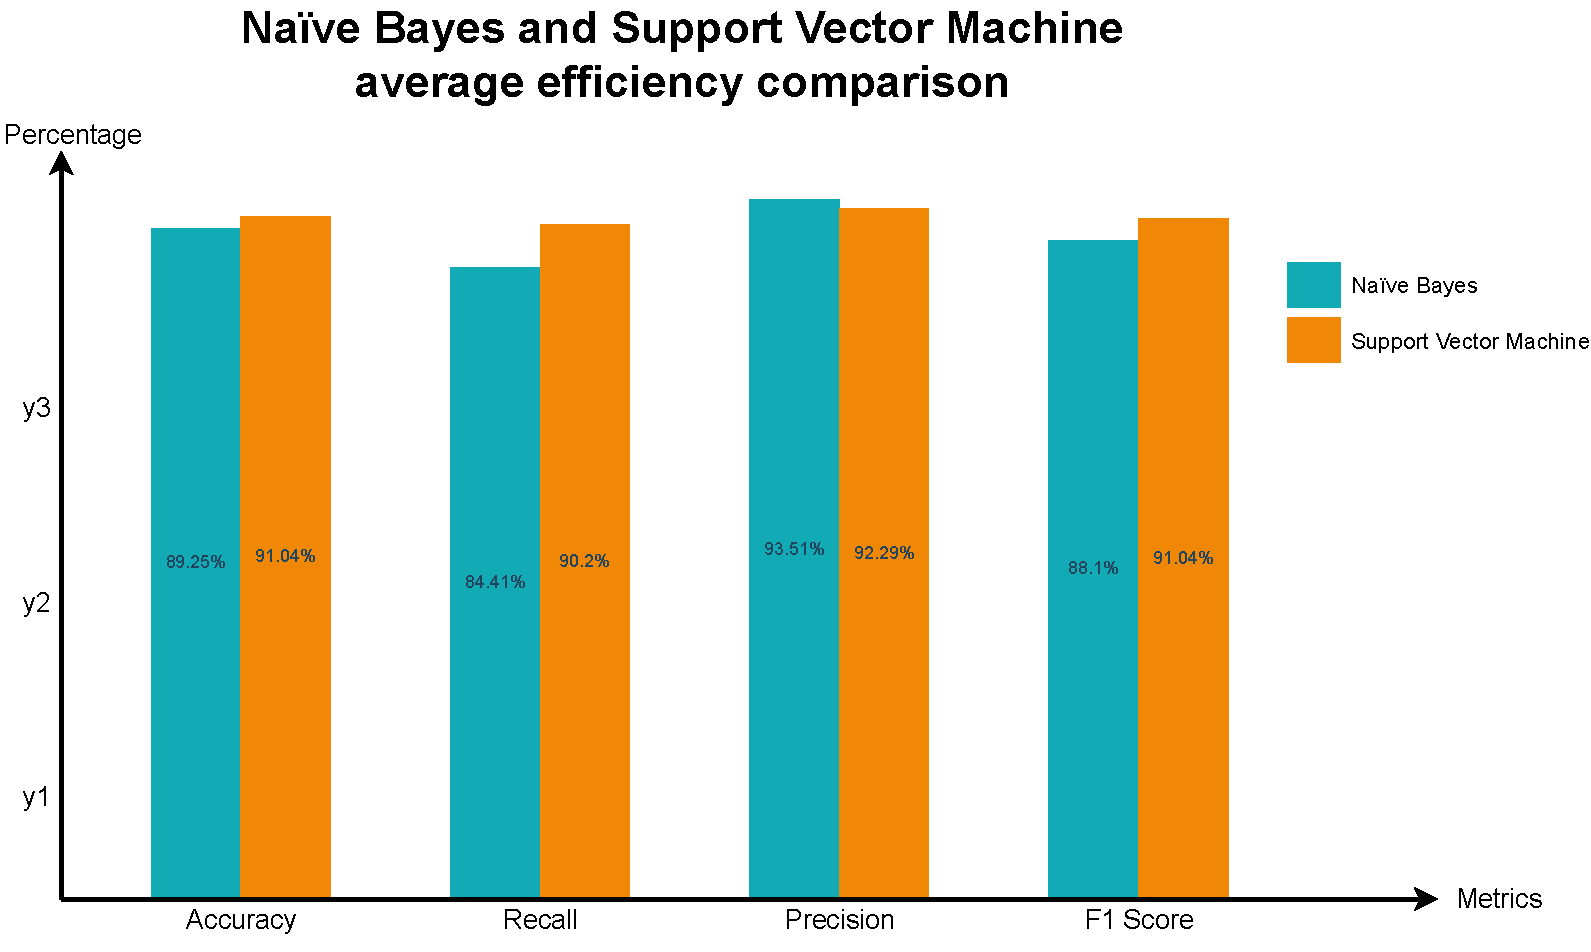
\includegraphics[scale=.35]{average.pdf}
\end{figure}
\end{frame}

\section{Discussion and conclusion}

\begin{frame}[fragile=singleslide]\frametitle{Discussion and conclusion}
\begin{itemize}[label=$\bullet$]
\item Conclusion of results
\item Comparing efficiency
\item Limitations
\item Future work
\end{itemize}
\end{frame}

\end{document}